\documentclass[11pt]{beamer}
\title{Local Reasoning about the Presence of Bugs:Incorrectness Separation Logic}
\usepackage{verbatim}
\usepackage{amsmath}
\usepackage{amsthm}
\usepackage{graphics}
\usepackage{color}
\usepackage{stmaryrd}
\usepackage{multicol}

\newtheorem{proposition}{Proposition}


%\author{Peter W. O'Hearn}
\date{\today}


\begin{document}
\maketitle
\begin{frame}\frametitle{Overview}
\begin{itemize}
\item A brief review of the incorrectness logic.
\item Introduction to separation logic.
\item ISL (incorrectness separation logic).
\item Investigation of the tool \textsc{Infer}.

\end{itemize}
\end{frame}

\begin{frame}\frametitle{Incorrectness Logic}

Let $\epsilon$ range over a collection of exit conditions, to include at lease ``ok" and ``er". An \textit{under-approximate triple} is of the form:
\[[p]C[\epsilon: q]\]
meaning q under-approximates the states when $C$ exits via $\epsilon$ starting form states in $p$.

Sometimes, we write $[p]C\color{teal}{[ok:q]}\color{red}{[er:r]}$ as shorthand for $[p]C\color{teal}{[ok:q]}$ and $[p]C\color{red}{[er:r]}$


An important point: the triple $[p]C[\epsilon: q]$ express the reachability property that involves termination. \textbf{Every state in the result is reachable from some states in the presumption}
\end{frame}

\begin{frame}\frametitle{Separation Logic}
Separation logic is an extension of Hoare logic, which employs novel logical operators and able to handle heap-manipulating programs with aliasing.

More types of variables: $x = 1 \text{ and } y\mapsto 1$
\begin{multicols}{2}
\begin{example}
$\{x\ne y, y \ne z, x\ne z\}$

$[x] = 1;$

$[y] = 2;$

$[z] = 3;$


$\{x\mapsto 1, y\mapsto 2 , x\mapsto 3\}$



\end{example}

\begin{example}
$\{x1\ne x2, x1 \ne x3, \cdots\}$

$[x1] = 1;$

$[x2] = 2;$

$\cdots$

$[xn] = n;$


$\{x1\mapsto 1, x2\mapsto 2 , \cdots , xn\mapsto n\}$



\end{example}

\end{multicols}
Therefore we introduce a new operator $\ast$ read as ``and seperately''.

$x1 \mapsto - \ast \cdots \ast xn \mapsto -$


$\forall x, v, v'. x\mapsto v \ast x\mapsto v' \Rightarrow \textbf{false}$

We also use $emp$ to represent the empty heap.
\end{frame}

\begin{frame}\frametitle{SL: Semantic}
\begin{center}
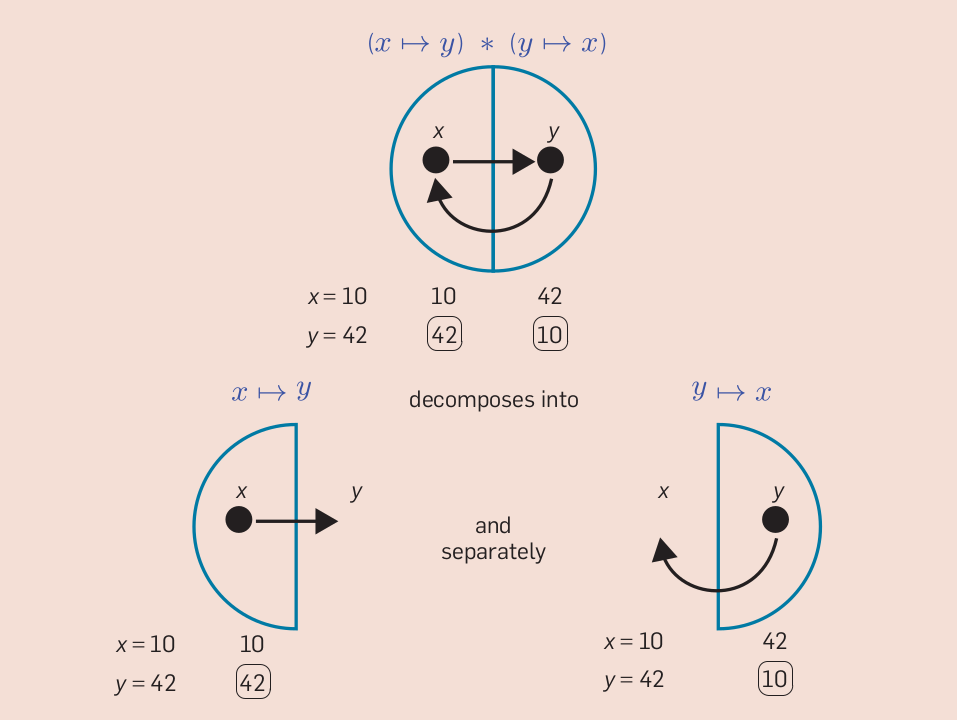
\includegraphics[scale=0.28]{picSema.png}
\end{center}
\end{frame}

\begin{frame}\frametitle{SL: Semantic}
Let $s: Vars \rightarrow Ints$ and  $h: Nats \rightarrow Ints$ be the ``store'' and ``heap''.

$s$ is similar to the evaluation.


\begin{center}
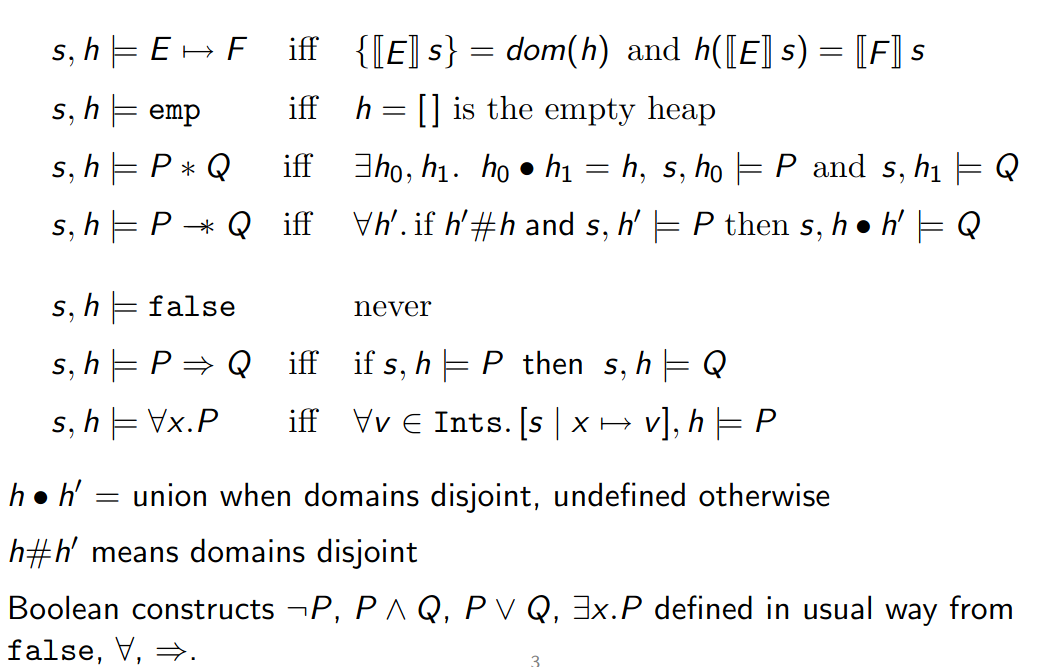
\includegraphics[scale=0.28]{matSema.png}
\end{center}
\end{frame}

\begin{frame}\frametitle{SL: Rules and Axioms}

\begin{center}
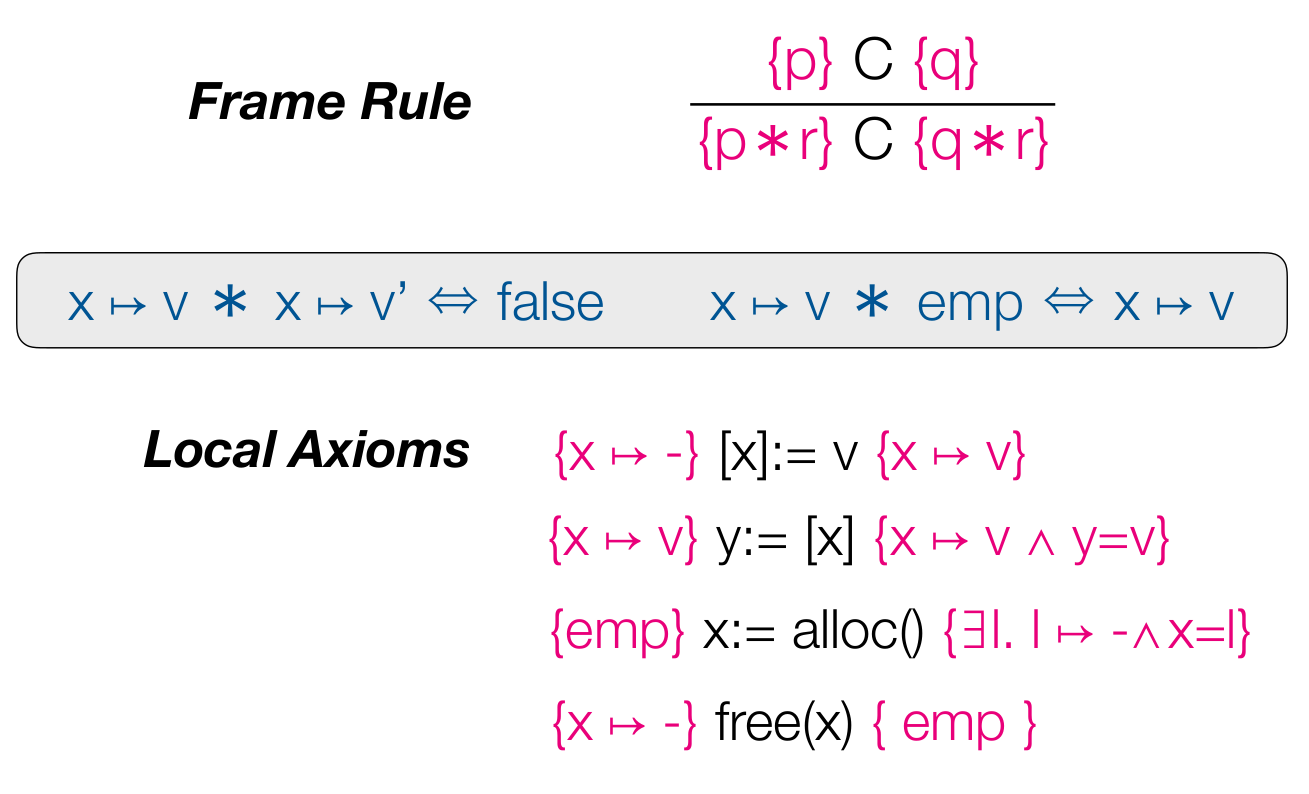
\includegraphics[scale=0.2]{separules.png}
\end{center}
The primitive statements of the language update or access only one memory cell each time. These local axioms are extremely concise and able to do local reasoning.

Frame rule allows to extend the reasoning from one cell to multiple cell. 
\end{frame}


\begin{frame}\frametitle{SL: Proof Example}
\begin{center}
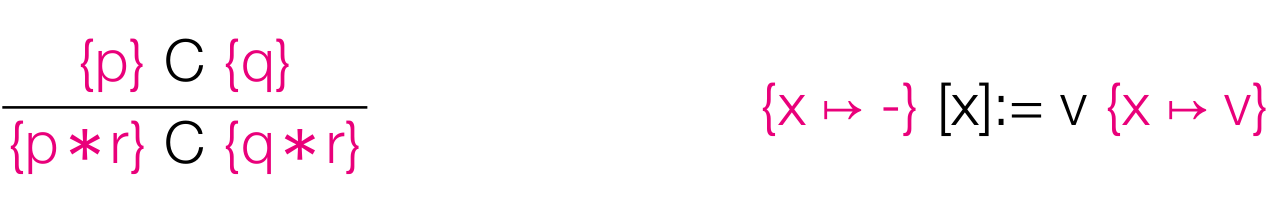
\includegraphics[scale=0.2]{rulesForExp.png}

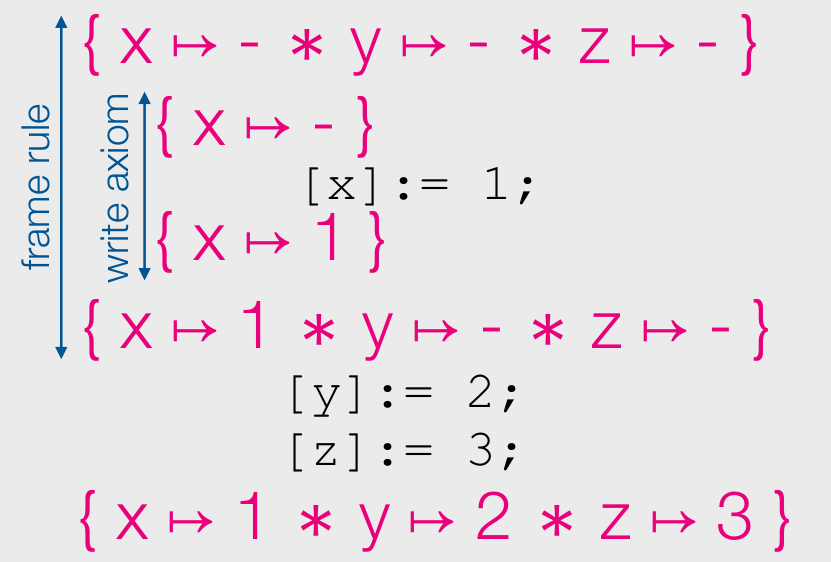
\includegraphics[scale=0.2]{proofExp.png}
\end{center}
\end{frame}

\begin{frame}\frametitle{SL: Soundness and Completeness}

\begin{theorem}[Soundness]
SL is sound:

\[\{p\}C\{q\} \text{ is provable} \Rightarrow \{p\}C\{q\} \text{ is true}\]
\end{theorem}

SL is not complete however.
\end{frame}


\begin{frame}\frametitle{Incompleteness: Example}
\begin{center}
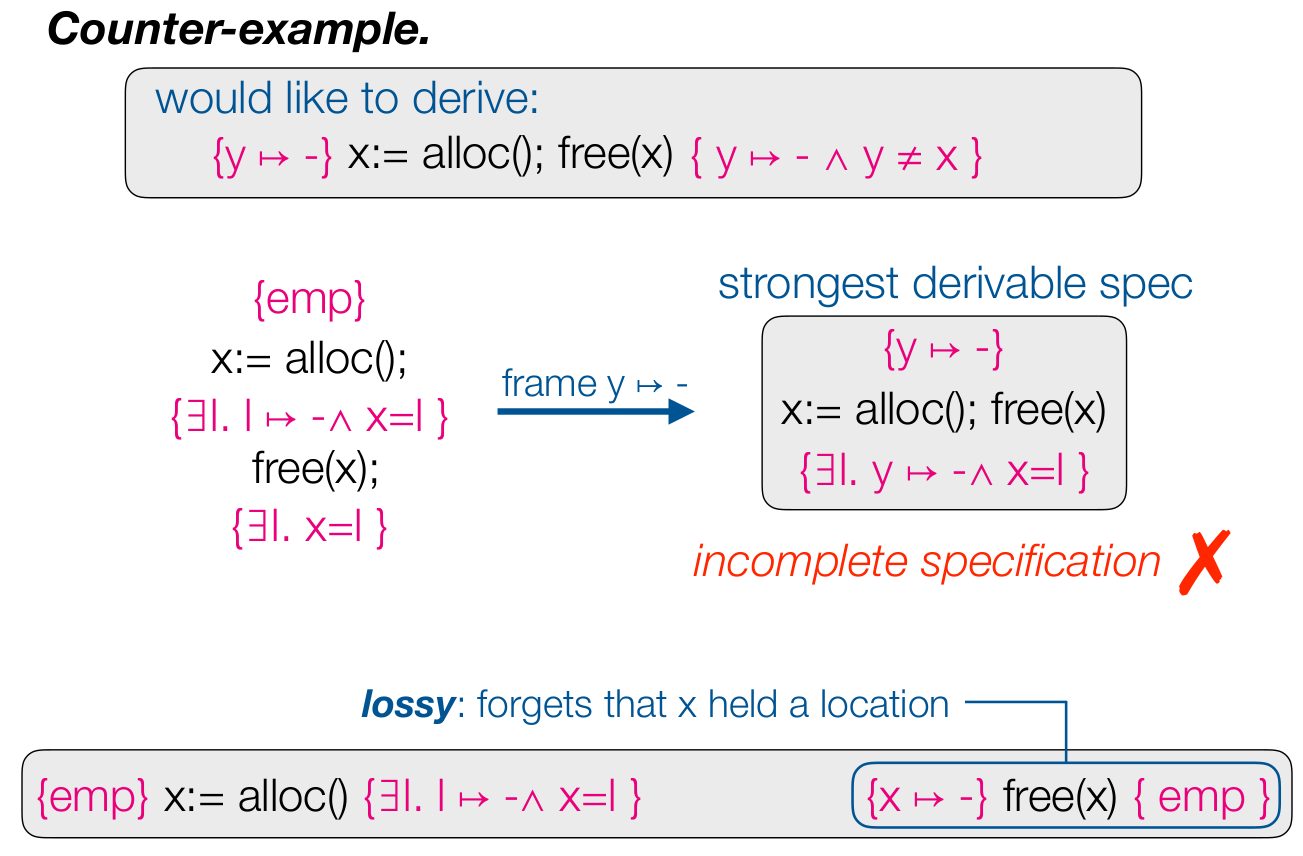
\includegraphics[scale=0.2]{incomplete.png}
\end{center}
\end{frame}

\begin{frame}\frametitle{ISL: Incorrectness Separation Logic}
\begin{center}
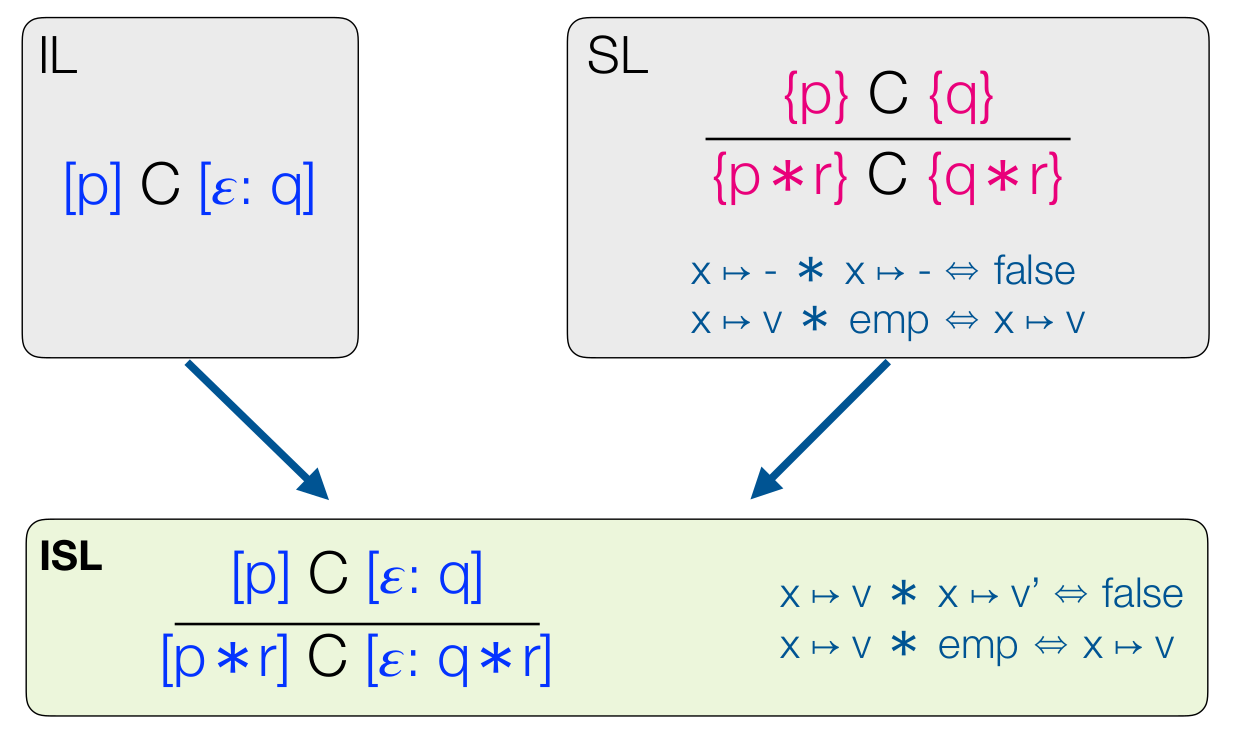
\includegraphics[scale=0.2]{isl.png}
\end{center}


\end{frame}


\begin{frame}\frametitle{ISL: Problem of Combining}

\begin{center}
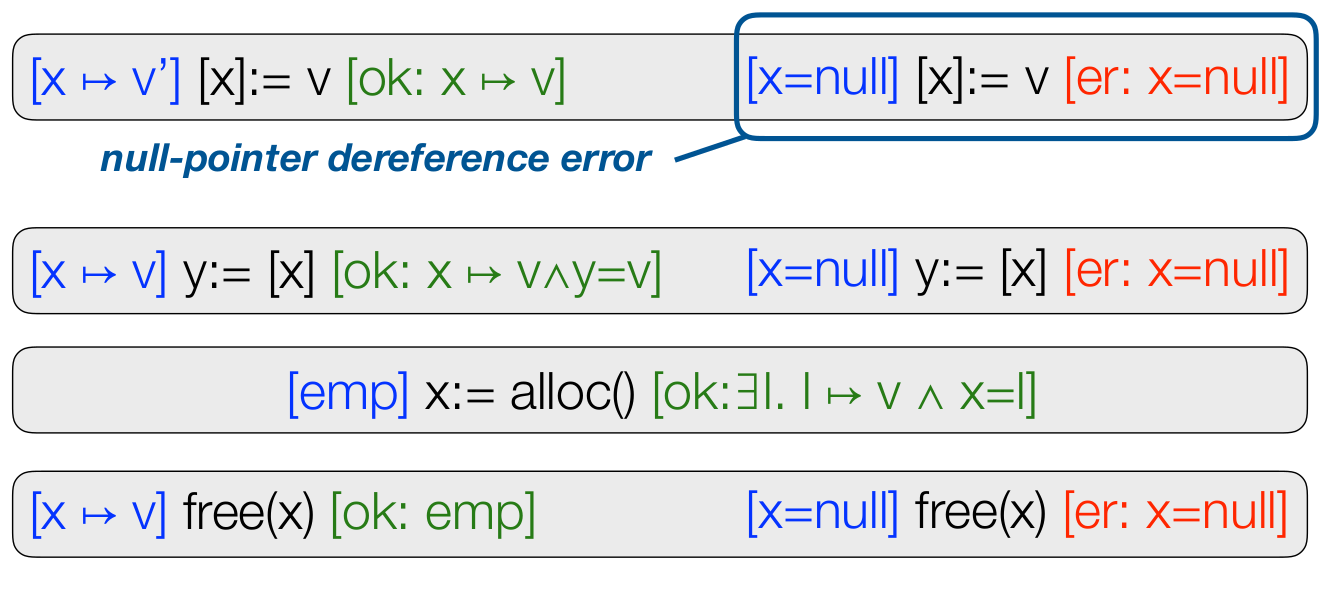
\includegraphics[scale=0.2]{firsttry.png}
\end{center}



\end{frame}

\begin{frame}\frametitle{ISL: Problems of Combining}

\begin{center}
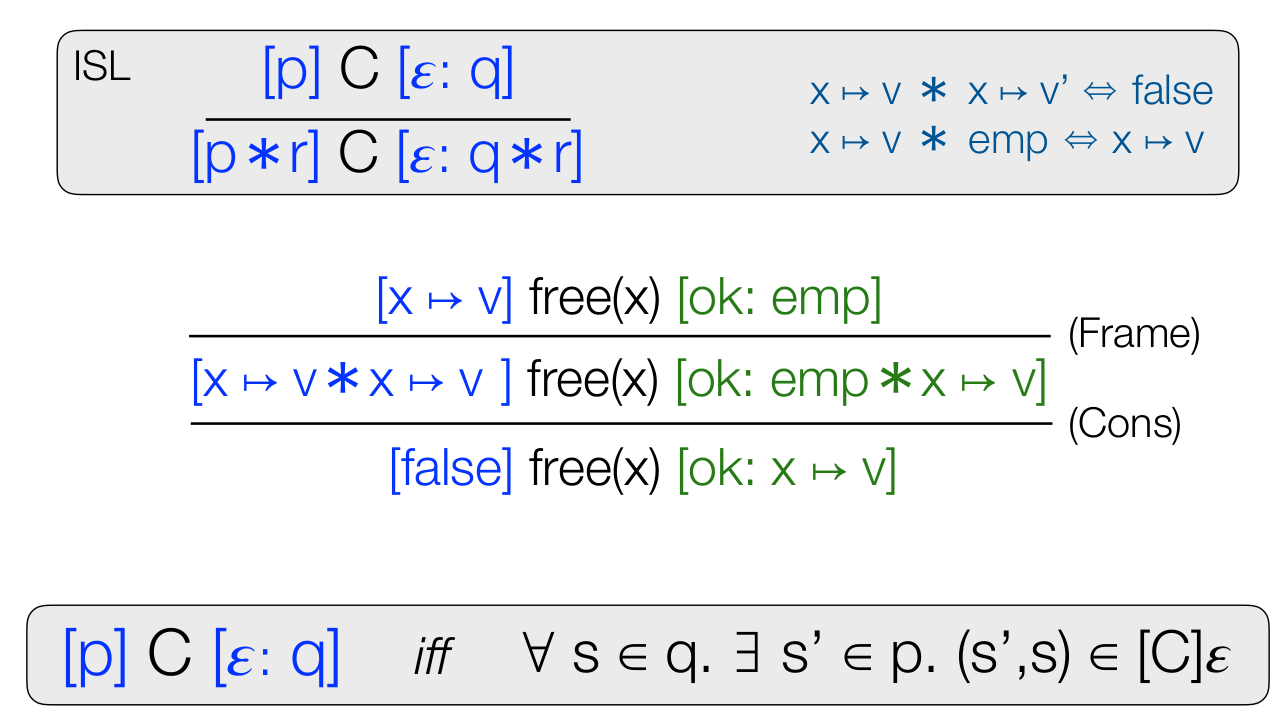
\includegraphics[scale=0.2]{kaboom.png}
\end{center}

\end{frame}

\begin{frame}\frametitle{ISL: Solution}
The solution for the frame rule is to remember that we allocated memory for the pointer even if we freed them.

\textbf{Old free rule:}

\[[x\mapsto v] free(x) [ok:emp]\]

\textbf{New free rule:}

\[[x\mapsto v] free(x) [ok:x\not\mapsto]\]

\begin{center}
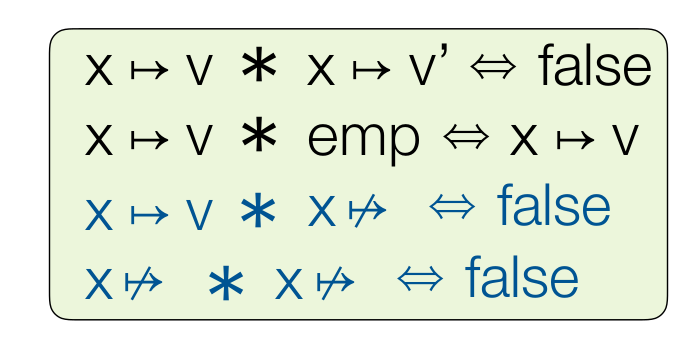
\includegraphics[scale=0.2]{compatible.png}
\end{center}
\end{frame}

\begin{frame}\frametitle{ISL: Target Programs and Rules}
\begin{center}
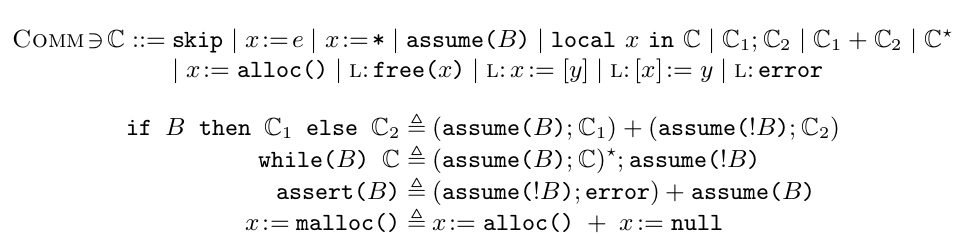
\includegraphics[scale=0.3]{program.png}

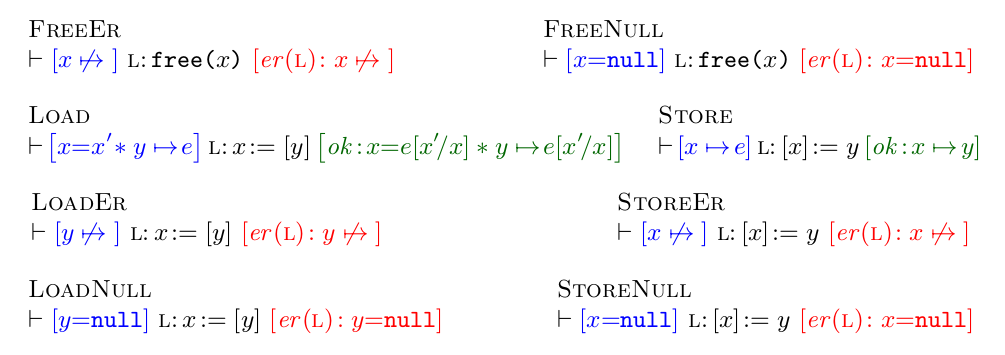
\includegraphics[scale=0.3]{error.png}
\end{center}
\end{frame}

\begin{frame}\frametitle{ISL: Semantic}
Adapt original semantic incorrectness logic to ISL semantic 
\begin{center}
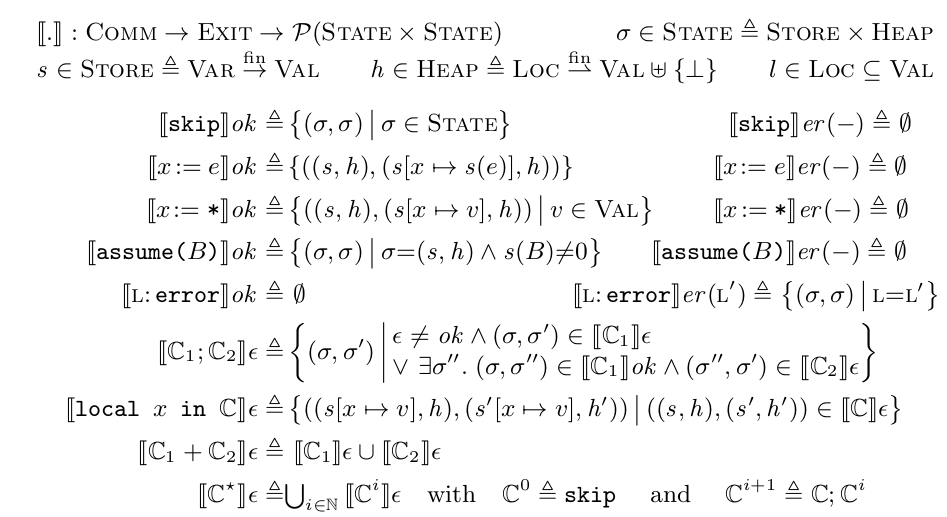
\includegraphics[scale=0.3]{adapt1.png}
\end{center}
\end{frame}



\begin{frame}\frametitle{ISL: Semantic}

Semantic related to memory operations.

\begin{center}
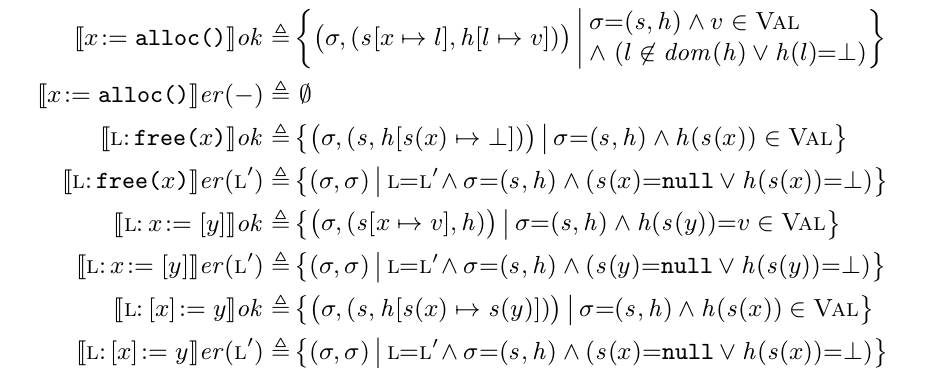
\includegraphics[scale=0.3]{adapt2.png}
\end{center}
\end{frame}

\begin{frame}\frametitle{ISL: Soundness}
\begin{theorem}[Soundness of ISL]
For all $p, \mathbb{C}, q, \epsilon$, if $\vdash [p]\mathbb{ C }[\epsilon:q]$, the $\models [p] \mathbb{C} [\epsilon: q]$.
\end{theorem}
The definition of $\models [p] \mathbb{C} [\epsilon: q]$ is $\forall \sigma_q\in q. \exists \sigma_p\in p. (\sigma_p, \sigma_q)\in [[\mathbb{C}]]\epsilon$
\end{frame}

\begin{frame}\frametitle{Tool: Infer}
Current Version: 0.17.0

Only able to do inference with separation logic.

\texttt{./infer run -- javac test.java}
\begin{multicols}{2}
\begin{center}
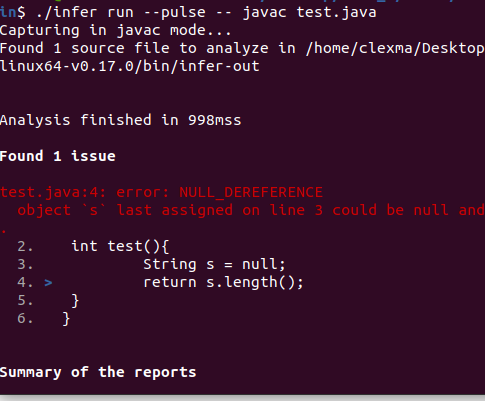
\includegraphics[scale=0.3]{result.png}

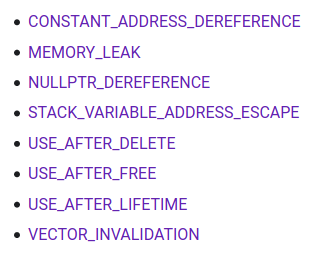
\includegraphics[scale=0.4]{types.png}
\end{center}
\end{multicols}
In the doc of next version:

\texttt{./infer --pulse --pulse-intraprocedural-only}
\end{frame}
\end{document}